%\documentclass{exam}
\documentclass[answers,addpoints]{exam}
\usepackage{amsmath,amssymb,enumerate,float,tikz,etoolbox,ifthen,xcolor,fullpage,ulem,graphicx, comment,hyperref,multicol,enumerate,makecell,pgfplots}
\pgfplotsset{compat=1.18}
\usetikzlibrary{decorations.pathreplacing}

\definecolor{MyGreen}{rgb}{0.1, 0.4, 0.1}
\definecolor{MyBlue}{rgb}{0.1, 0.1, 0.9}

\AtBeginEnvironment{solution}{\color{MyGreen}}

\newboolean{NoSolutions}

\newcommand\pts[1][2]{\textcolor{MyBlue}{\text{\bf [#1 pts]}}}
\newcommand\pt{\textcolor{MyBlue}{\text{\bf [1 pt]}}}
\newcommand\ds{\displaystyle}

\makeatletter
\renewcommand{\thefigure}{\thequestion.\arabic{figure}}
\@addtoreset{figure}{question}
\makeatother

\setlength\parindent{0in}
\pagestyle{empty}
\begin{document}

\section*{MATH 100 GROUP PROJECT 2: \\Implicit Differentiation and Linear Approximation}

\normalsize

\subsection*{Contributors}

Alexandre \textbf{Boutoille} (22291660) Brennan \textbf{Coetzer} (64702178) Dino \textbf{Lee} (29709300) Andaya \textbf{Vincent} (33234436)

\hrulefill

\subsection*{Reflection Question}

\begin{solution}
  Enter your solution here
\end{solution}

\hrulefill

\newpage

\fullwidth{
\subsection*{Assignment questions}}

\begin{questions}
  \question \
  \begin{solution}

    \begin{figure}[H]
      \centering
      \begin{tabular}{@{}l@{}}
        $\displaystyle x^3+y^3=6xy$ \\[6pt]
        $\displaystyle (3)^3+(3)^3=6(3)(3)$ \\[6pt]
        $\displaystyle 54=54$ \\[12pt]
        $\displaystyle \frac{d}{dx}3x^2+\frac{dy}{dx}3y^2=\frac{d}{dx}6y+\frac{dy}{dx}6x$ \\[6pt]
        $\displaystyle \frac{dy}{dx}=\frac{2y-x^2}{y^2-2x}$ \\[6pt]
        $\displaystyle \frac{dy}{dx}=\frac{2(3)-(3)^2}{(3)^2-2(3)}$ \\[6pt]
        $\displaystyle =-1$ \\[12pt]
        $\displaystyle y-y_{1}=m(x-x_{1})$ \\[6pt]
        $\displaystyle y-3=-1(x-3)$ \\[6pt]
        $\displaystyle y=-x+6$ \\[6pt]
      \end{tabular}
      \caption{Question 1a Mathematical Work}
      \label{fig:1a-math}
    \end{figure}

    % As seen in \ref{fig:1a-math}...

    We can assume that we can write y=f(x) near this point as if point (3,3) exists, and only has one tangent line value that exists. While on the graph there may be two points at the x value 3, at the point (3,3), y=f(x) locally exists. If we could not write y=y(x) near this point, the slope of our tangent line wouldn't exist, and would be a value of $\infty$, signaling the graph turning back on itself at this specific point. However, since the slope of the tangent line is -1, which is a real number, we can say that y=f(x) near (3,3). Even though the overall curve fails the vertical line test, in this small defined region, there is only one tangent line that exists; therefore, we can say y=f(x) near (3,3).

    \begin{figure}[H]
      \centering
      \begin{tabular}{@{}l@{}}
        $\displaystyle L(x)=f(a)+f^\prime(a)(x-a)$ \\[6pt]
        $\displaystyle L(1)=3-1(1-3)$ \\[6pt]
        $\displaystyle L(2.5)=3-1(2.5-3)$ \\[6pt]
        $\displaystyle =3.5$ \\[6pt]
      \end{tabular}
      \caption{Question 1b Mathematical Work}
      \label{fig:1b-math}
    \end{figure}

    The single step estimate for b is inaccurate since linear approximations are approximations, and the farther you go away from the point for which the linear approximation was derived from, the less accurate the approximation becomes. Essentially what linear approximations does is find points that are on the tangent line; this is why the farther away you go, the less accurate it becomes, unless it is a function like a sin wave where the tangent line will intersect with the function's graph again. Regardless, since the curve in this case is concave down (as we can see from the plot of the curve), we know that the actual value of the graph when x=2.5 will be less than that of its linear approximation at (3,3). That is why the linear approximation is an overestimate.

  \end{solution}

  % -------------------------------------------------------

  \question \
  \begin{solution}

    \begin{figure}[H]
      \centering
      \begin{tabular}{r r r r r r}
        \hline
        \multicolumn{1}{c}{$n$} &
        \multicolumn{1}{c}{$x_n$} &
        \multicolumn{1}{c}{$y_n$} &
        \multicolumn{1}{c}{$m_n$} &
        \multicolumn{1}{c}{$x_{n+1}$} &
        \multicolumn{1}{c}{$y_{n+1}$} \\
        \hline
        0 & 3.0000 & 3.0000 & -1.0000 & 2.9000 & 3.1000 \\
        1 & 2.9000 & 3.1000 & -0.5801 & 2.8000 & 3.1580 \\
        2 & 2.8000 & 3.1580 & -0.3485 & 2.7000 & 3.1929 \\
        3 & 2.7000 & 3.1929 & -0.1886 & 2.6000 & 3.2117 \\
        4 & 2.6000 & 3.2117 & -0.0658 & 2.5000 & 3.2183 \\
        5 & 2.5000 & 3.2183 & 0.0348 & 2.4000 & 3.2148 \\
        \hline
      \end{tabular}
      \caption{a Calculations Table}
      \label{fig:2a-vi-table}
    \end{figure}

    \begin{figure}[H]
      \centering
      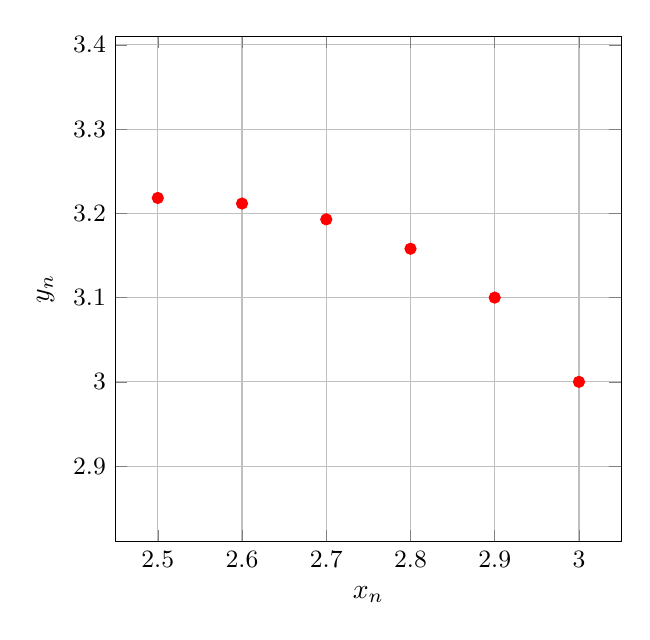
\begin{tikzpicture}
        \begin{axis}[
            axis equal,
            xlabel=$x_n$,
            ylabel=$y_n$,
            grid=both,
            width=8cm,
            height=8cm,
            xmin=2.45, xmax=3.05,
            ymin=3.0, ymax=3.22,
            tick label style={font=\small}
          ]

          \addplot[only marks, red, mark=*] coordinates {
            (3.0000, 3.0000)
            (2.9000, 3.1000)
            (2.8000, 3.1580)
            (2.7000, 3.1929)
            (2.6000, 3.2117)
            (2.5000, 3.2183)
          };
        \end{axis}
      \end{tikzpicture}
      \caption{a $x_n$ vs $x_y$ plot}
      \label{fig:2a-vii-plot}
    \end{figure}

    The approximate value for b produced in this process is $b \approx 3.218927$, this is slighter closer to the actual value than the value of $3.5$ obtained in Question 1. The accuracy improved because a new tangent line is used every time we move closer to $2.5$ from $3$. However, as we are approximating the value of $y_n+1$ using mn, the tangent line still slightly overshoots the actual value of $y_n+1$ of the curve for every step, resulting in error. These errors then accumulate, resulting in an approximate value of $b$ that is higher than the actual value.

    \begin{figure}[H]
      \centering
      \begin{tabular}{r r r r r r}
        \hline
        \multicolumn{1}{c}{$n$} &
        \multicolumn{1}{c}{$x_n$} &
        \multicolumn{1}{c}{$y_n$} &
        \multicolumn{1}{c}{$m_n$} &
        \multicolumn{1}{c}{$x_{n+1}$} &
        \multicolumn{1}{c}{$y_{n+1}$} \\
        \hline
        0 & 3.0000 & 3.0000 & -1.0000 & 2.9500 & 3.0500 \\
        1 & 2.9500 & 3.0500 & -0.7649 & 2.9000 & 3.0882 \\
        2 & 2.9000 & 3.0882 & -0.5976 & 2.8500 & 3.1181 \\
        3 & 2.8500 & 3.1181 & -0.4689 & 2.8000 & 3.1416 \\
        4 & 2.8000 & 3.1416 & -0.3646 & 2.7500 & 3.1598 \\
        5 & 2.7500 & 3.1598 & -0.2772 & 2.7000 & 3.1737 \\
        6 & 2.7000 & 3.1737 & -0.2018 & 2.6500 & 3.1837 \\
        7 & 2.6500 & 3.1837 & -0.1354 & 2.6000 & 3.1905 \\
        8 & 2.6000 & 3.1905 & -0.0761 & 2.5500 & 3.1943 \\
        9 & 2.5500 & 3.1943 & -0.0223 & 2.5000 & 3.1954 \\
        10 & 2.5000 & 3.1954 & 0.0270 & 2.4500 & 3.1941 \\
        \hline
      \end{tabular}
      \caption{b Calculations Table}
      \label{fig:2b-table}
    \end{figure}

    \begin{figure}[H]
      \centering
      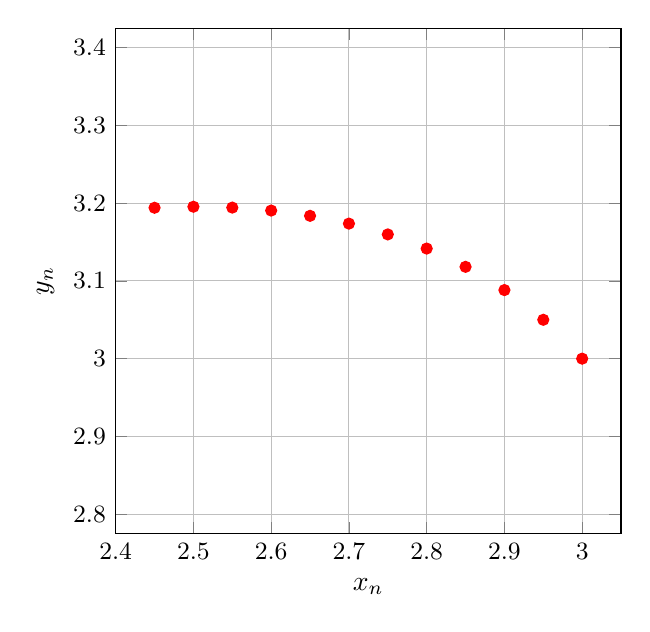
\begin{tikzpicture}
        \begin{axis}[
            axis equal,
            xlabel=$x_n$,
            ylabel=$y_n$,
            grid=both,
            width=8cm,
            height=8cm,
            xmin=2.40, xmax=3.05,
            ymin=3.0, ymax=3.20,
            tick label style={font=\small}
          ]

          \addplot[only marks, red, mark=*] coordinates {
            (3.0000, 3.0000)
            (2.9500, 3.0500)
            (2.9000, 3.0882)
            (2.8500, 3.1181)
            (2.8000, 3.1416)
            (2.7500, 3.1598)
            (2.7000, 3.1737)
            (2.6500, 3.1837)
            (2.6000, 3.1905)
            (2.5500, 3.1943)
            (2.5000, 3.1954)
            (2.4500, 3.1941)
          };
        \end{axis}
      \end{tikzpicture}
      \caption{b $x_n$ vs $x_y$ plot}
      \label{fig:2b-plot}
    \end{figure}

    Changing $h$ from $0.1$ to $0.05$ caused the approximate value of $b$ to go from $b \approx 3.218927$ to $b \approx 3.195442$. This is even closer to the actual value of $b \approx 3.174607$, meaning that using a smaller $h$ improved the accuracy of the approximation.

    This is because we must calculate a new $y_n$ more frequently when using a smaller $h$, thus each tangent line calculated is closer to the curve and the error produced on each step becomes smaller. This results in a smaller error overall and thus a closer approximation to the actual value of $b$.

  \end{solution}

  %\hrulefill
  % -------------------------------------------------------
  \question \
  \begin{solution}

    \begin{figure}[H]
      \centering
      \begin{tabular}{@{}l@{}}
        $\displaystyle \frac{dy}{dx}=\frac{2(0)-(0^2)}{(0)^2-2(0)}$ \\[6pt]
        $\displaystyle =0=\text{DNE}$ \\[6pt]
      \end{tabular}
      \caption{Question 3a Mathematical Work}
      \label{fig:3a-math}
    \end{figure}

    At $(0,0)$, multiple paths pass-through. It's a point of self-intersection, so has no (WORD). $\therefore$ we can't reliably use the tangent line method.

    The derivative found in \ref{fig:1a-math} can't really be simplified at $(0,0)$ using L'Hôpital's rule as seen in \ref{fig:3a-math}. $\therefore$ you cannot get a slope for the tangent line, so the iterative tangent line method at $(0,0)$ can't be used.

    A linear approximation cannot be used to find $(p,q)$ when $q=1$ at $(0,0)$. This is because the slope of the tangent line is an indeterminate form, as there is an intersection of paths at $(0,0)$ on the graph. We cannot use iterative tangent line techniques to estimate anything if we start at $(0,0)$, as the initial slope is an indeterminate form.

    Since no singular tangent line exists at $(0,0)$ when the graph intersects, as there are multiple paths leading to $(0,0)$, issues will arise when solving for the slope.

    There are essentially multiple tangent lines at $(0,0)$ since multiple path lead there. This means there are multiple coordinates that the linear approximation could give at this point for $(a,b)$ when $a=1$, and $(p,q)$ with $q=1$. Generally, you cannot apply this approaching starting at $(0,0)$.

  \end{solution}

  % -------------------------------------------------------

  \hrulefill
  % -------------------------------------------------------

  % -------------------------------------------------------

\end{questions}
\end{document}

%-------------------------------------------------------------
%-------------------------------------------------------------
%-------------------------------------------------------------
